% !TeX root = scaffold-70.tex
\renewcommand{\imagepath}{../70-supervised/img}

\chapter{Supervised Analysis: Zero-Shot Classification}\label{ch:supervised}
In this chapter, the newspaper articles \todo{continue}

\section{Analysis Procedure}
In contrast to topic modelling, in the case of zero-shot classification (see section~\ref{ch:zero_shot}) training and optimization has already been performed by the model provider. The employed BART model~\autocite{lewis_bart_2020} \todo{decide for one kind of reference} is not trained on any inputs and is not altered during the classification process. It can assign a relative semantic proximity $p_{i, l}$ to a given newspaper article $i$ for each label $l$ out of a set of labels. This probability represents how close the meaning of the label is to the meaning of the article. Similar to the procedure in topic modelling, a label was assigned to an article if it had the highest proximity:
\begin{align}
    l_{i} = \max_{l'} p_{i, l'}
\end{align}
Also like in the topic modelling procedure, the information-theoretical entropy for each articles was calculated as~\autocite{gray_entropy_2013}
\begin{align}
    H_i = -\sum_{l'} p_{i, l'} \ln p_{i, l'}.
\end{align}
Low entropy signifies that the model could attest a very close proximity of one of the labels, hence an unambiguous assignment of label, whereas a high value of $H_i$ testifies an ambiguous association between the article and the label. As the range of $H$ depends on the number $n_\text{labels}$ of labels, the following normalized variant is used for comparing the model's security across categories:
\begin{align}
    \widetilde{H}_i = \frac{H_i}{\ln n_\text{labels}}
\end{align}

In order to examine the articles properties with respect to topic, sentiment, delinquency, and journalistic style, as has been motivated in section~\ref{ch:this_thesis}, for each of these categories a list of labels was compiled based on the author's intuition of the category and on what would seem interesting for the analysis of role model qualities. The labels used in the analysis are presented in section~\ref{ch:supervised_results} for each category.

\begin{figure}
    \centering
    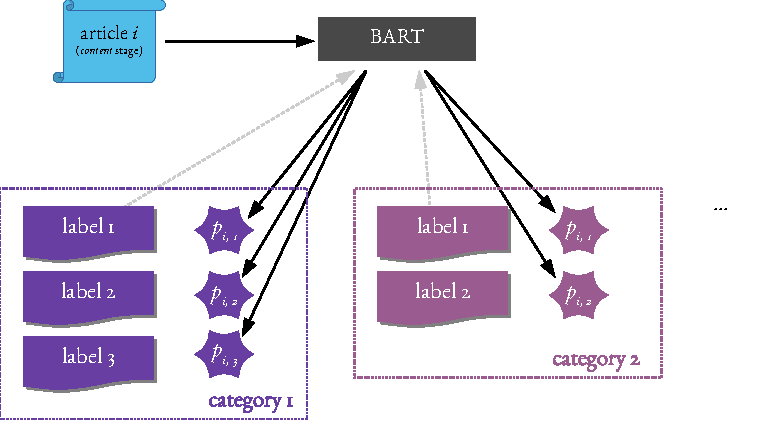
\includegraphics[]{\imagepath/zero_shot_schema.pdf}
    \caption{Schematic of the zero shot classification procedure: An article $i$ is fed into the BART model along with a set of labels, called a category. BART then assigns a relative proximity $p$ to each label for this article. This is repeated for different categories, each having a different set of labels. The BART model itself doesn't depend on any input and is not altered during the whole process.}\label{fig:zero_shot_schema}
\end{figure}

The classification procedure is illustrated in figure~\ref{fig:zero_shot_schema}. The BART model was integrated as suggested in \textcite{huggingfacebart-large-mnli_facebookbart-large-mnli_nodate}. As an input to the model the text in the \textit{content} stage was used, i.e. with most structure of the human language preserved.

\section{Results}\label{ch:supervised_results}
\begin{table}
    \centering
    \resizebox{0.88\textwidth}{!}{../../../build/thesis/70-supervised/zero_shot_result_table.tex}
    \caption{Results of the zero-shot classification for each category along with $\chi^2$ contingency and per-label tests. Legend: $\Braket{\widetilde{H}}$ is the average of the normalized entropy $\widetilde{H}$.}\label{tab:zero_shot_result_table}
\end{table}
\paragraph{Topics}
\paragraph{Sentiment}
\paragraph{Relatability}
\paragraph{Delinquency}
\paragraph{Newspaper Coverage}

\section{Discussion}